\tikzstyle{spring}=[thick, decorate,decoration={zigzag,pre length=1.5mm,post
        length=1.5mm,segment length=6}]

\begin{figure}[H]
    \centering %图片居中
    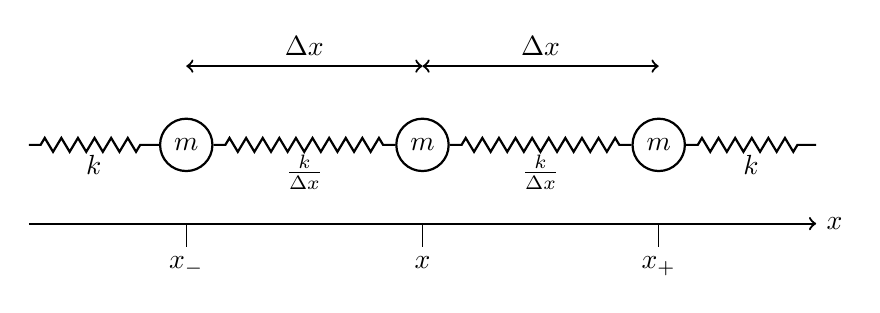
\begin{tikzpicture}
        \node[circle,draw=black,thick] (b1) at (2,0){$m$};
        \node[circle,draw=black,thick] (b2) at (5,0){$m$};
        \node[circle,draw=black,thick] (b3) at (8,0){$m$};

        \draw[spring](0,0)--(b1)node[midway,below]{$k$};
        \draw[spring](b1)--(b2)node[midway,below]{$\frac{k}{\Delta x}$};
        \draw[spring](b2)--(b3)node[midway,below]{$\frac{k}{\Delta x}$};
        \draw[spring](b3)--(10,0)node[midway,below]{$k$};

        \draw[->,thick](0,-1)--(10,-1) node[right]{$x$};
        \draw (2,-1)--(2,-1.3) node[anchor=north]{$x_-$};
        \draw (5,-1)--(5,-1.3) node[anchor=north]{$x$};
        \draw (8,-1)--(8,-1.3) node[anchor=north]{$x_+$};
        \draw [<->,thick](2,1)--(5,1) node[midway,above]{$\Delta x$};
        \draw [<->,thick](5,1)--(8,1) node[midway,above]{$\Delta x$};
    \end{tikzpicture}
    \caption{無限長線性彈簧} %最终文档中希望显示的图片标题
\end{figure}